\documentclass{article}
\usepackage{graphicx,xy,amsmath,amssymb,amsthm,physics,mathtools,tcolorbox,hyperref}
\usepackage{xepersian}
\settextfont{XB Niloofar}
\title{	
	پیش گزارش هفتم درس آزمایشگاه اپتیک - دکتر مهدوی
	\\
	\small
	موضوع آزمايش: بررسی نور قطبیده شده روی يک دی الکتريک و مقايسه
	نتايج آن با معادلات فرنل
}
\author{
حسین محمدی 
\\
۹۶۱۰۱۰۳۵
}
\begin{document}
\maketitle
\section{شرایط قطبیده شدن نور هنگام انعکاس از سطح}
می دانیم که ضرایب بازتاب برای مولفه های موازی و عمودی یک پرتو نور، مساوی نیستند و این باعث می شود که قطبش نور در بازتاب از یک سطح تغییر کند. این بنیان و اساسی است که در بررسی این پدیده و آزمایش بایستی در خاطر داشته باشیم. 

\noindent
پدیده ای که بروستر آن را مشاهده کرد این بود که اگر نور با زاویه خاصی 
($\theta_B$)
به مرز بین دو محیط شفاف برخورد کند، به طور کامل از سطح محیط شفاف عبور می کند؛ همچنین نور بازتابیده به طور کامل قطبیده می شود. (مطابق رابطه ۷-۷ دستور کار یعنی زاویه بین میدان الکتریکی نور بازتابیده و بردار عمود بر سطح صفر می شود یا ضرایب بازتاب برای دو مولفه مساوی می شود.) یا معادلا  راستای انتشار پرتو بازتاب شده و راستای پرتو شکست یافته، بر هم عمود باشند.

\noindent
با قرار دادن 
$\alpha=0$ 
در رابطه ۷-۷ دستور کار، دقیقا روابط ساده شده ی اسنل به دست می آید.
\[
n_1 \sin(\theta_1) =  n_2 \sin(\theta_2) \ \ \ \ \ \ \ \ \ \ \ \tan(\theta_B) = \frac{n_2}{n_1}
\]


سودمندی این فرآیند این است که می توان از سطوحی که دارای ضریب شکست مختلف هستند، به عنوان یک قطبشگر استفاده کرد.
\section{رسم رابطه 7-7 دستور کار بر حسب 
$\theta$
و تفسیر آن
}
\begin{figure}[h]
	\centering
	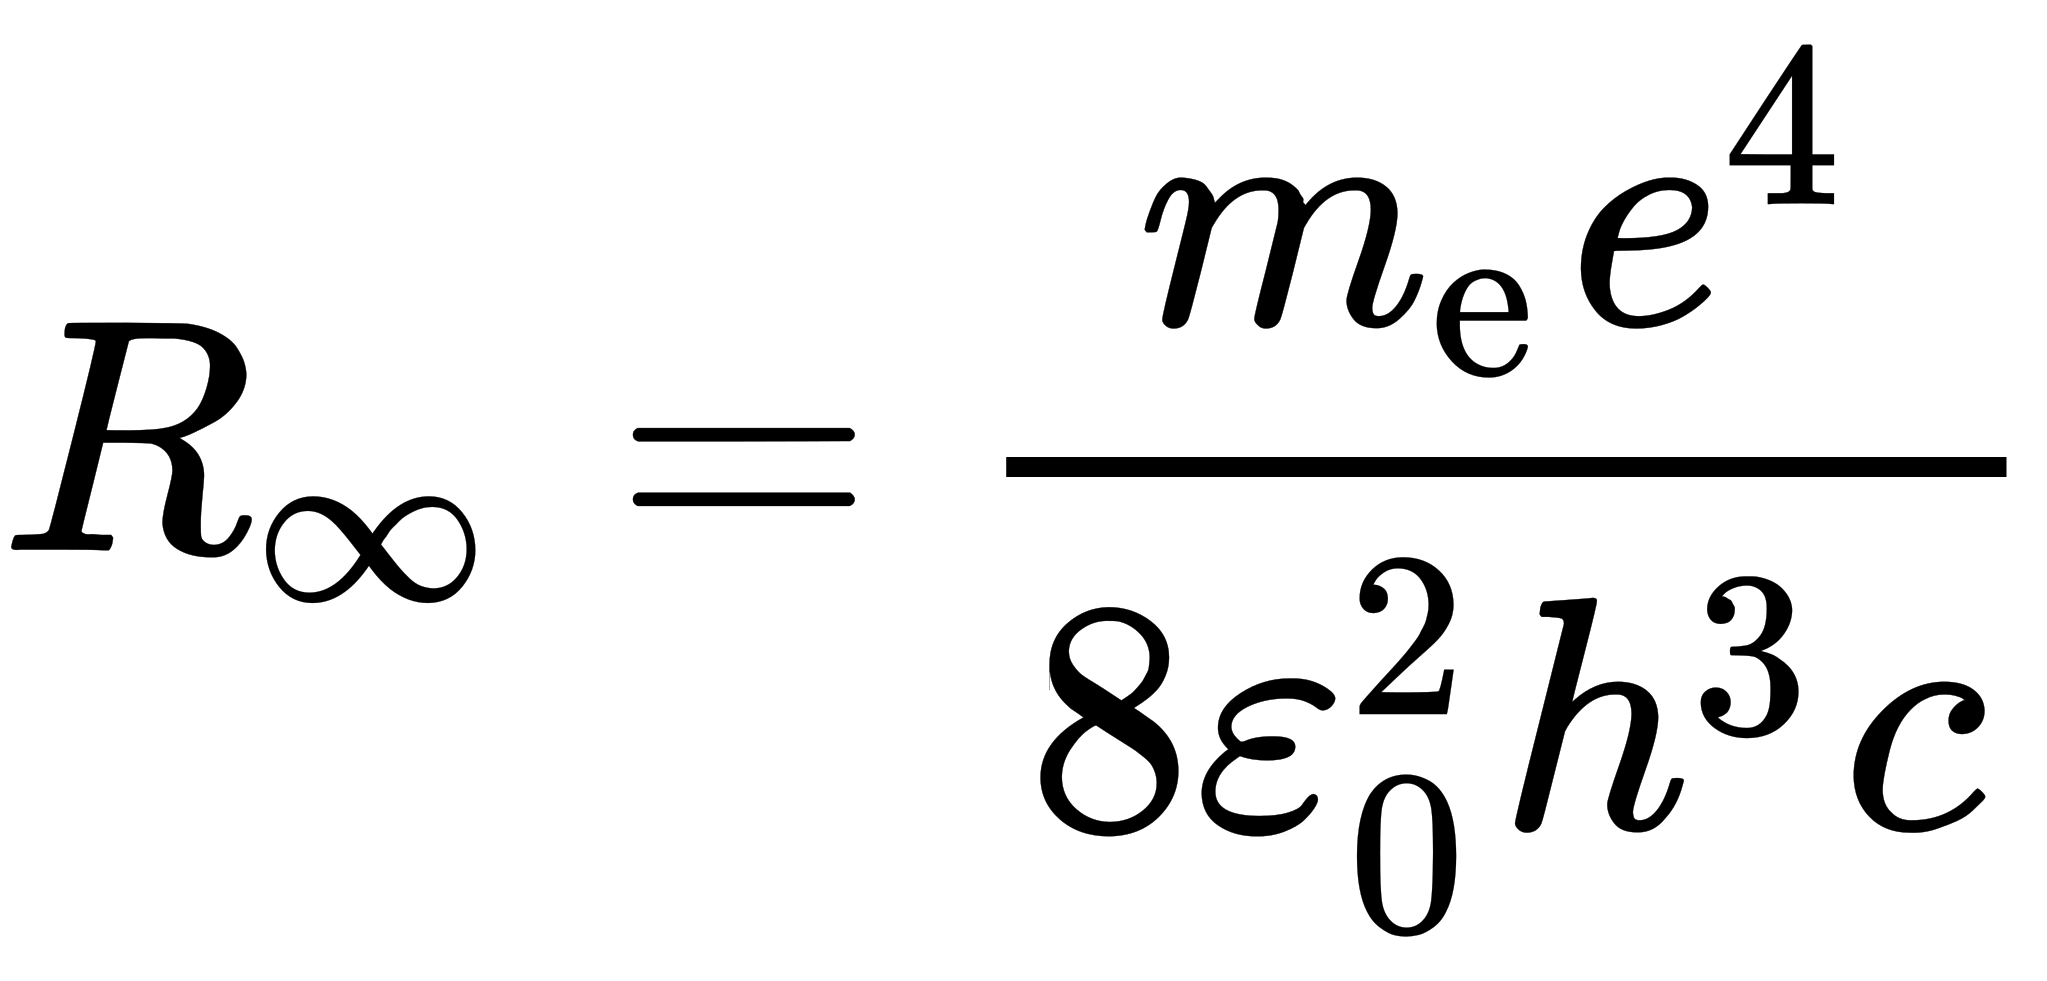
\includegraphics[scale=0.8]{1.jpg}
	\caption{نمودار
$\tan (\alpha)$
بر حسب 
$\theta$
مطابق رابطه ۷-۷	
}
	\label{Fig1}
\end{figure}
برای ضریب شکست های مختلف نمودار را در شکل 
\ref{Fig1}
می بینیم.(نمودار از بالا به پایین رسم شده است یعنی بالاترین نمودار دارای ضریب شکست ۱ است و همینطور پایین می آید.)

\noindent
جاهایی که مقدار $\tan (\alpha)$ صفر شده است را پیدا کنیم، مقدار $\theta$ متناظر آن ها همان زاویه ی بروستر است. پس نتیجه این است که هرچه ضریب شکست بیشتر شود، زاویه ی بروستر هم بیشتر می شود.















\end{document}ظ